\begin{figure*}%
	\centering%
	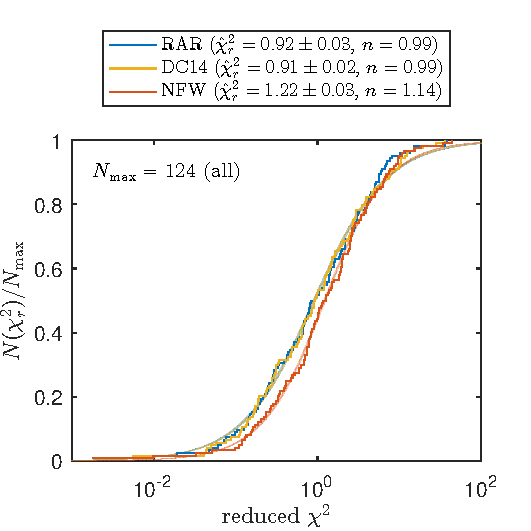
\includegraphics[width=0.33\hsize]{\ROOTPATH/all.pdf}%
	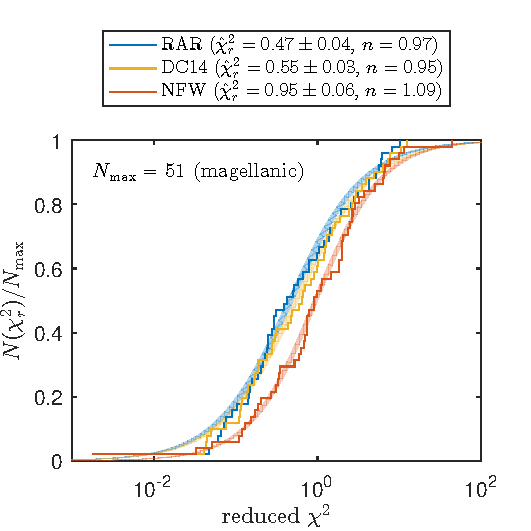
\includegraphics[width=0.33\hsize]{\ROOTPATH/magellanic.pdf}%
	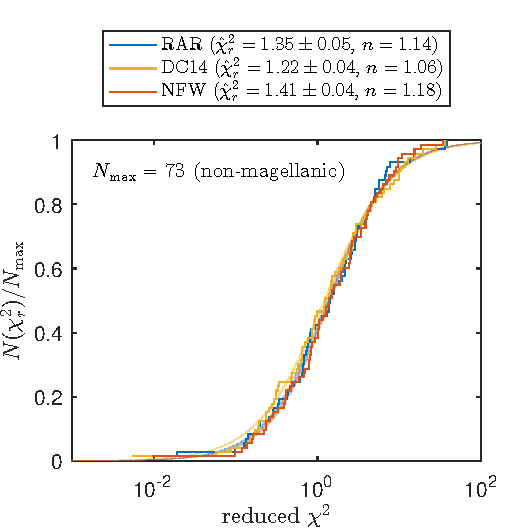
\includegraphics[width=0.33\hsize]{\ROOTPATH/nonmagellanic.pdf}%
	\caption{Goodness of model analysis for all galaxy types (left), only magellanic (middle) and non-magellanic (right). We count the population of fitted galaxies having a reduced $\chi^2$ smaller than a given one. The normalized population may be well described by the function $1/[1 + (\chi_r^2/\hat\chi_r^2)^{-n}]$ with the median $\hat\chi_r^2$ and the supplemental descriptor $n$. RAR and DC14 are similarly good when the galaxy type is ignored. NFW, in contrast, is clearly disfavored here. This picture becomes much more obvious when only magellanic types are considered. On the other hand, focusing on non-magellanic types there is no clear favorite.}%
	\label{fig:gof-stairs}
\end{figure*}